% !TEX encoding = UTF-8
% !TEX TS-program = pdflatex
% !TEX root = ../tesi.tex

\subsection{UC2 - Lettura dati da CD}
\begin{itemize}
  \item \textbf{Identificativo}: UC2
  \item \textbf{Nome}: lettura dati da CD
  \item \textbf{Descrizione grafica}:
\end{itemize}

\begin{figure}[h]
  \centering
  %  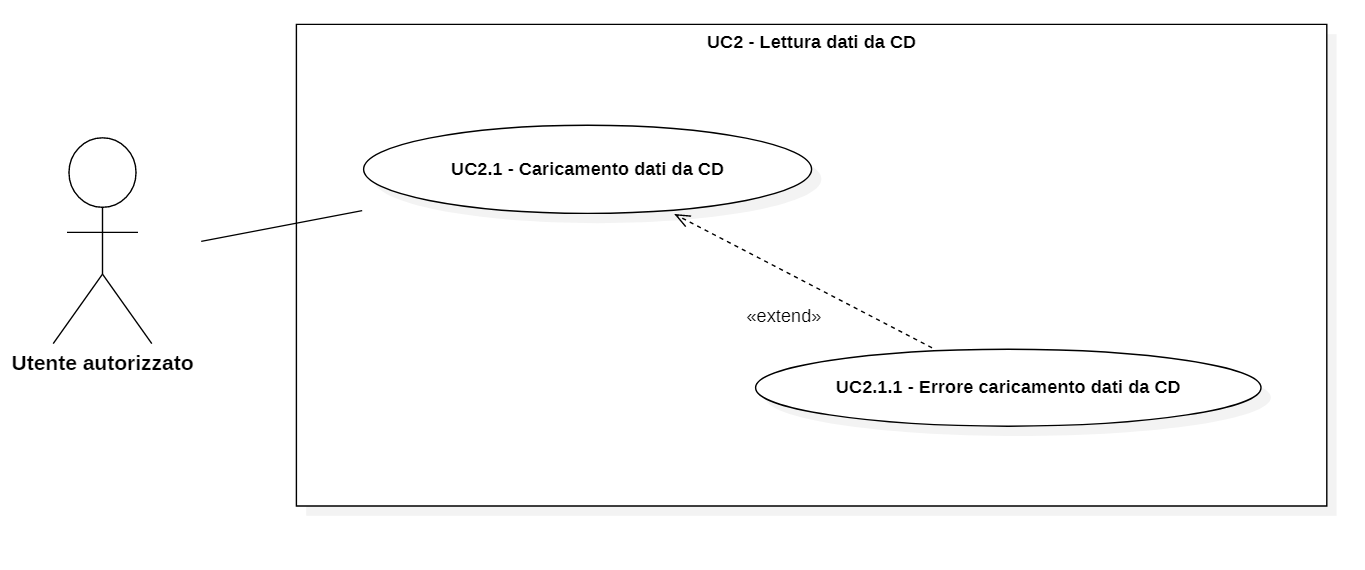
\includegraphics[scale=0.50]{images/UC2.png}
  \caption{Descrizione grafica caso d'uso UC2}
\end{figure}

\begin{itemize}
  \item \textbf{Attori}
        \begin{itemize}
          \item \textit{Primari}: utente autorizzato
        \end{itemize}
  \item \textbf{Precondizione}: l'utente autorizzato si trova nella pagina per il caricamento dei dati.
  \item \textbf{Postcondizione}: l'utente visualizza i dati che ha caricato.
  \item \textbf{Scenario principale}: l'utente premendo sull'apposito bottone può caricare i file contenuti nel CD di interesse.
  \item \textbf{Scenario secondario}: il sistema riscontra un errore nella procedura di caricamento dei dati. (\textbf{UC2.1})
\end{itemize}

\subsubsection{UC2.1 - Errore caricamento dati da CD}
\begin{itemize}
  \item \textbf{Identificativo}: UC2.1
  \item \textbf{Nome}: errore caricamento dati da CD
  \item \textbf{Descrizione grafica}: (approfondita in UC2)
  \item \textbf{Attori}
        \begin{itemize}
          \item \textit{Primari}: utente autorizzato
        \end{itemize}
  \item \textbf{Precondizione}: l'utente ha tentato di caricare i dati.
  \item \textbf{Postcondizione}: l'errore viene mostrato all'utente.
  \item \textbf{Scenario principale}: il sistema non è riuscito a gestire la richiesta di caricamento dei dati da parte dell'utente.
\end{itemize}